\documentclass[../master/master.tex]{subfiles}
\begin{document}
\todo[inline]{Here and throughout: Smaller figures, thicker lines, use different marker for the different algorithms. One might view this in black\& white printout, or be color blind. It is good to have these in minds whenever you present plots}

In this section, we look at how the theoretical analysis of the algorithms relates to how the algorithms perform in practice. We investigate which algorithm performs faster, both in terms of symbolic steps, as well as runtime. From the theoretical analysis of complexity, we expect that the linear-time algorithm should perform less symbolic steps. Since Lockstep is the algorithm used in practice, based on \todo{citation}, we predict that the lockstep algorithm will perform better time-wise. We hope to test whether our predictions are correct and find the most effective version of the algorithms.

In order to do this, we have collected a set of graphs of different number of nodes, diameter, interconnectivity, or number of SCCs. Most of these graphs are from the VLTS benchmark suite \cite{vlts} and two of them are from Stanford Large Network Dataset Collection \cite{snapnets}. An overview of the graphs can be seen in Table \ref{graphs}. 
 
We want to find out whether the number of nodes, the diameter or how interconnected the graph is has an influence on which algorithm works best, or if there is one algorithm superior to the others.

To measure the performance of the algorithms, we count the number of symbolic steps each algorithm performs, and furthermore note the time it took to run the algorithm. Here, we do not record how long it took to read a graph file and load it into a BDD, but only record the time in which the algorithm is actually doing work.\todo{which machine was it run on?}

We have tested our implementations of the linear-time and Lockstep algorithms as descried in the papers \cite{linear}\cite{lockstep}, as well as our modification of the two using trimming and of lockstep using edge restriction. The data can be seen in Figures \ref{timeres} and \ref{stepres}.

\subsection{Edge Restriction}
As edge restriction only improves the runtime of the Lockstep algorithm, and does not change the number of symbolic steps performed, we have pltted Lockstep and Lockstep with edge restriction on a graph of their own (Figure \ref{er graph}). Here, we look at the time it takes per symbolic step in relation to the number of nodes. As can be seen below, the effect of edge restriction is not clear, as there is no significant change in performance for better or worse. Even though we hoped that edge restriction woudl improve the runtime, we can now see that it can be quite a heavy, and therefore time consuming operation on some graphs.

Since edge restriction does not change the number of symbolic steps in comparison to the vanilla lockstep, we will not be comparing it in the graphs below with the rest of the algorithms.
\begin{figure}[h!]
  \centering
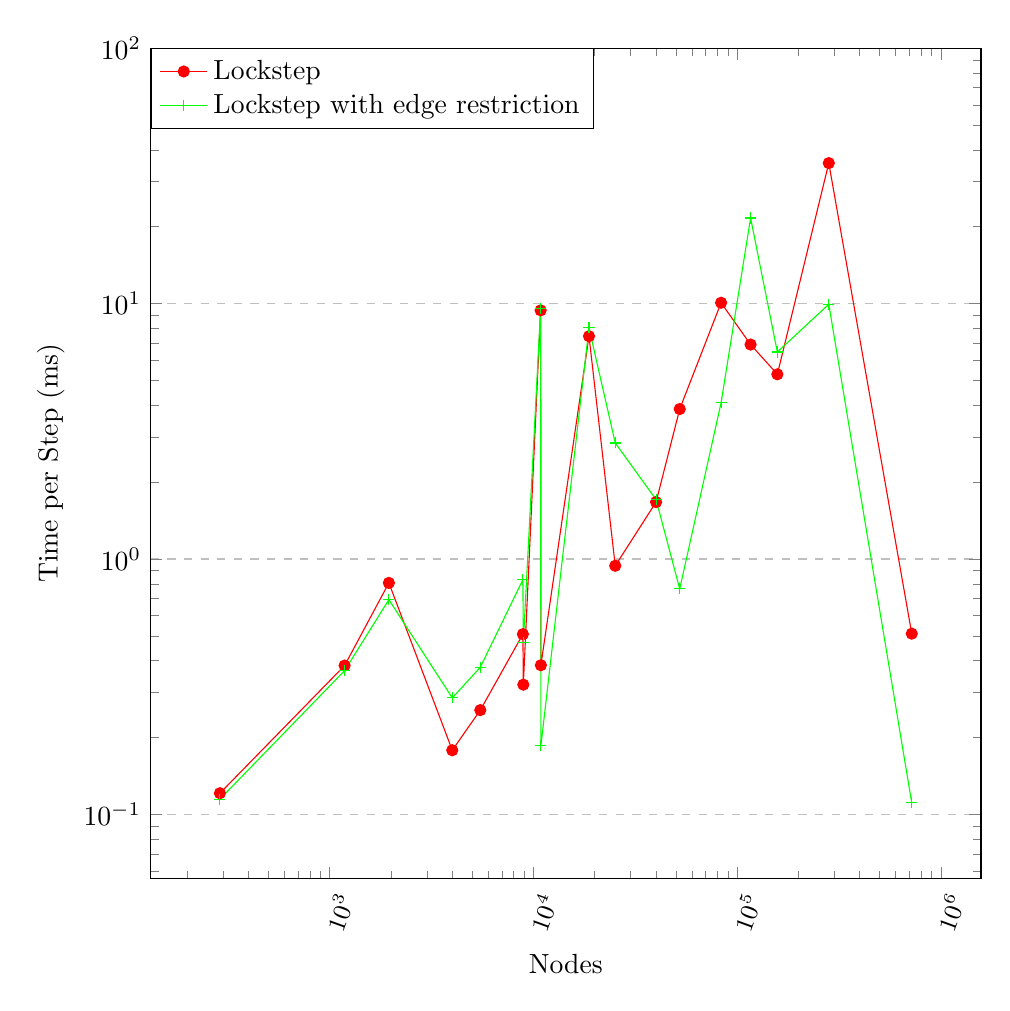
\begin{tikzpicture}
\begin{axis}[
height = \textwidth,
width=\textwidth,
x tick label style = {font = \small, align = center, rotate = 70, anchor = north east},
% title={Small graphs},
xlabel={Nodes},
ylabel={Time per Step (ms)},
ymin=0, ymax=100,
legend style={at={(0,1)}, anchor=north west,legend cell align=left},
ymajorgrids=true,
grid style=dashed,
ymode=log,
log basis y={10},
xmode=log,
log basis x={10},
% xtick ={289, 1183, 1952, 3996, 5486, 8879, 8921, 10849, 10879, 18746, 25217, 40006, 52268, 83436, 116456, 157604, 281903, 720247 }
]
\addplot[color=red,mark=*,]coordinates {(289, 0.12111801242236025)(1183, 0.38285714285714284)(1952, 0.8064516129032258)(3996, 0.17842842842842843)(5486, 0.2561816652649285)(8879, 0.5080408092685458)(8921, 0.3222929141716567)(10849, 9.40983606557377)(10879, 0.3839806192747369)(18746, 7.455172413793103)(25217, 0.9411309830669786)(40006, 1.6711202209696168)(52268, 3.866146656134808)(83436, 10.077079107505071)(116456, 6.913526727731424)(157604, 5.286887325488905)(281903, 35.49112943426139)(720247, 0.5103813966709304)};
\addplot[color=green,mark=+,]coordinates {(289, 0.11490683229813664)(1183, 0.3657142857142857)(1952, 0.6935483870967742)(3996, 0.28603603603603606)(5486, 0.3771236333052986)(8879, 0.8307107037869618)(8921, 0.4714321357285429)(10849, 9.573770491803279)(10879, 0.18555530320236202)(18746, 8.03448275862069)(25217, 2.8472657334337947)(40006, 1.709689917636325)(52268, 0.7638559768299105)(83436, 4.0912778904665315)(116456, 21.634155463527748)(157604, 6.464333223621054)(281903, 9.944128919433526)(720247, 0.11100312396367173)};

\legend{Lockstep, Lockstep with edge restriction}
\end{axis}
\end{tikzpicture}
\caption{Comparison for time taken per step for vanilla and ER Lockstep.} \label{er graph}
\end{figure}

\subsection{Nodes vs. Steps}
We started by comparing the symbolic steps and number of nodes in the graph, as the complexity of the algorithms in Theorems \ref{linear} and \ref{lockstep} was described in terms of these two. Figure \ref{steps} shows that there is a somewhat positive correlation between number of nodes and symbolic steps, with some outliers. This is most likely due to the strengthened bound described in Theorem \ref{magic}. This will be tested in a later experiment.

The effect of trimming on the number of steps can be seen in this graph - it tends to help significantly is some cases, and even when it doesn't help, it doesn't harm the performance either.
\begin{figure}[h!]
  \centering
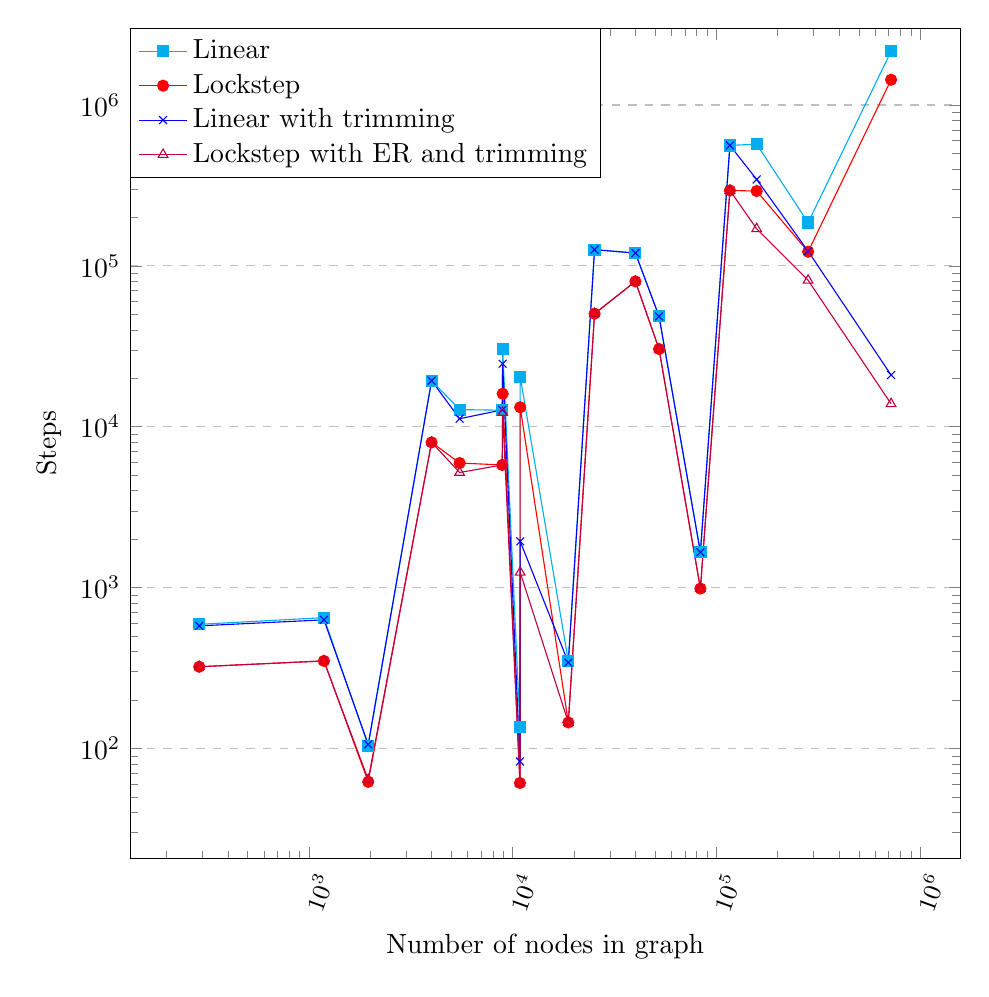
\begin{tikzpicture}
\begin{axis}[
height = \textwidth,
width=\textwidth,
x tick label style = {font = \small, align = center, rotate = 70, anchor = north east},
xlabel={Number of nodes in graph},
ylabel={Steps},
ymin=0, ymax=3000000,
legend style={at={(0,1)},anchor=north west,legend cell align=left},
ymajorgrids=true,
grid style=dashed,
ymode=log,
log basis y={10},
xmode=log,
log basis x={10},
%xtick={289, 1183, 1952, 3996, 5486, 8879, 8921, 10849, 10879, 18746, 25217, 40006, 52268, 83436, 116456, 157604, 281903, 720247}
]
\addplot[color=cyan,mark=square*,]coordinates {(289, 591)(1183, 650)(1952, 104)(3996, 19344)(5486, 12773)(8879, 12664)(8921, 30529)(10849, 136)(10879, 20434)(18746, 349)(25217, 126083)(40006, 120017)(52268, 48495)(83436, 1661)(116456, 560414)(157604, 570525)(281903, 185712)(720247, 2156545)};

\addplot[color=red,mark=*,]coordinates {(289, 322)(1183, 350)(1952, 62)(3996, 7992)(5486, 5945)(8879, 5783)(8921, 16032)(10849, 61)(10879, 13209)(18746, 145)(25217, 50434)(40006, 80011)(52268, 30384)(83436, 986)(116456, 294114)(157604, 291672)(281903, 122371)(720247, 1435356)};

\addplot[color=blue,mark=x,]coordinates {(289, 578)(1183, 630)(1952, 106)(3996, 19332)(5486, 11211)(8879, 12716)(8921, 24640)(10849, 83)(10879, 1938)(18746, 342)(25217, 126075)(40006, 120019)(52268, 48497)(83436, 1658)(116456, 560411)(157604, 344348)(281903, 123330)(720247, 20945)};

% \addplot[color=orange,mark=+,]coordinates {(289, 322)(1183, 350)(1952, 62)(3996, 7992)(5486, 5945)(8879, 5783)(8921, 16032)(10849, 61)(10879, 13209)(18746, 145)(25217, 50434)(40006, 80011)(52268, 30384)(83436, 986)(116456, 294114)(157604, 291672)(281903, 122371)(720247, 1435356)};

\addplot[color=purple,mark=triangle,]coordinates {(289, 322)(1183, 350)(1952, 64)(3996, 7990)(5486, 5191)(8879, 5783)(8921, 12264)(10849, 61)(10879, 1243)(18746, 145)(25217, 50432)(40006, 80013)(52268, 30386)(83436, 986)(116456, 294114)(157604, 169828)(281903, 81275)(720247, 13872)};

\legend{Linear, Lockstep, Linear with trimming, Lockstep with ER and trimming}
\end{axis}
\end{tikzpicture}
\caption{Symbolic steps compared to number of nodes} \label{steps}
\end{figure}
\todo[inline]{fix blank space}
\subsection{Nodes vs. Time}
Since the first comparison didn't give us much new insight), we decided to also compare the number of nodes to the time it takes to find SCCs, as we think of it as a quite impotant measure in practice. This graph (Figure \ref{time}  showed a stronger positive correlation. We noticed that for both small and large grpahs, the linear-algorithm tends to take less time to run, however both algorithms perform slightly randomly the larger the graphs get. This may be due to how interconnected they are or the number of SCCs in them, however we did not investigate this further.

From the graph, we can see that trimming not only has a positive effect on steps, but also on the runtime, or at least doesn't slow it down.
\begin{figure}[h!]
  \centering
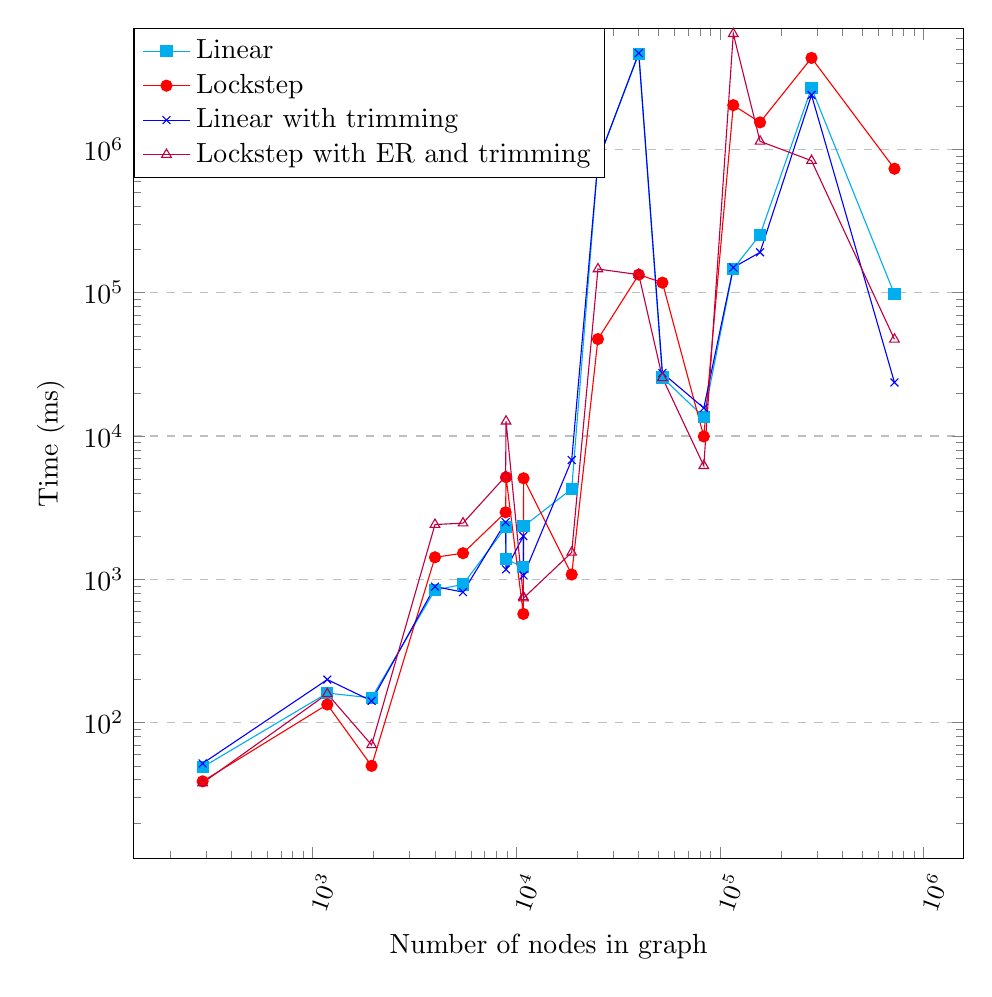
\begin{tikzpicture}
\begin{axis}[
height = \textwidth,
width=\textwidth,
x tick label style = {font = \small, align = center, rotate = 70, anchor = north east},
xlabel={Number of nodes in graph},
ylabel={Time (ms)},
ymin=0, ymax=7000000,
legend style={at={(0,1)},anchor=north west,legend cell align=left},
ymajorgrids=true,
grid style=dashed,
ymode=log,
log basis y={10},
xmode=log,
log basis x={10},
%xtick = {289, 1183, 1952, 3996, 5486, 8879, 8921, 10849, 10879, 18746, 25217, 40006, 52268, 83436, 116456, 157604, 281903, 720247}
]
\addplot[color=cyan,mark=square*,]coordinates {(289, 49)(1183, 161)(1952, 149)(3996, 843)(5486, 922)(8879, 2305)(8921, 1386)(10849, 1213)(10879, 2343)(18746, 4279)(25217, 823968)(40006, 4646640)(52268, 25608)(83436, 13562)(116456, 146786)(157604, 253563)(281903, 2675628)(720247, 97531)};

\addplot[color=red,mark=*,]coordinates {(289, 39)(1183, 134)(1952, 50)(3996, 1426)(5486, 1523)(8879, 2938)(8921, 5167)(10849, 574)(10879, 5072)(18746, 1081)(25217, 47465)(40006, 133708)(52268, 117469)(83436, 9936)(116456, 2033365)(157604, 1542037)(281903, 4343085)(720247, 732579)};

\addplot[color=blue,mark=x,]coordinates {(289, 52)(1183, 200)(1952, 142)(3996, 891)(5486, 815)(8879, 2505)(8921, 1174)(10849, 2005)(10879, 1066)(18746, 6804)(25217, 827718)(40006, 4694944)(52268, 27534)(83436, 15691)(116456, 149855)(157604, 191313)(281903, 2394077)(720247, 23638)};
%\addplot[color=orange,mark=+,]coordinates {(289, 37)(1183, 128)(1952, 43)(3996, 2286)(5486, 2242)(8879, 4804)(8921, 7558)(10849, 584)(10879, 2451)(18746, 1165)(25217, 143599)(40006, 136794)(52268, 23209)(83436, 4034)(116456, 6362908)(157604, 1885465)(281903, 1216873)(720247, 159329)};
\addplot[color=purple,mark=triangle,]coordinates {(289, 38)(1183, 159)(1952, 70)(3996, 2413)(5486, 2468)(8879, 5250)(8921, 12674)(10849, 755)(10879, 741)(18746, 1542)(25217, 146235)(40006, 133621)(52268, 25463)(83436, 6205)(116456, 6409803)(157604, 1137648)(281903, 834071)(720247, 47275)};
\legend{Linear, Lockstep,  Linear with trimming, Lockstep with ER and trimming}
\end{axis}
\end{tikzpicture}
\caption{Time taken to run algorithms} \label{time}
\end{figure}

\subsection{SCCs vs Steps}
The next comparison that seemed obvious to us was to compare if there was a correlation between the number of SCCs in the graph and the amount of steps it took to find them. While running some preliminary tests, we seemed to notice that the more SCCs the graph had, the longer time it would take. As can be seen in Figure \ref{stepscc}, there is a very obvious positive correlation. However, there is an outlier. This was a fairly large graph with only one SCC consisting of almost all of the graph's nodes, meaning that it took more steps than it would have to find a small SCC.
\begin{figure}[h!]
  \centering
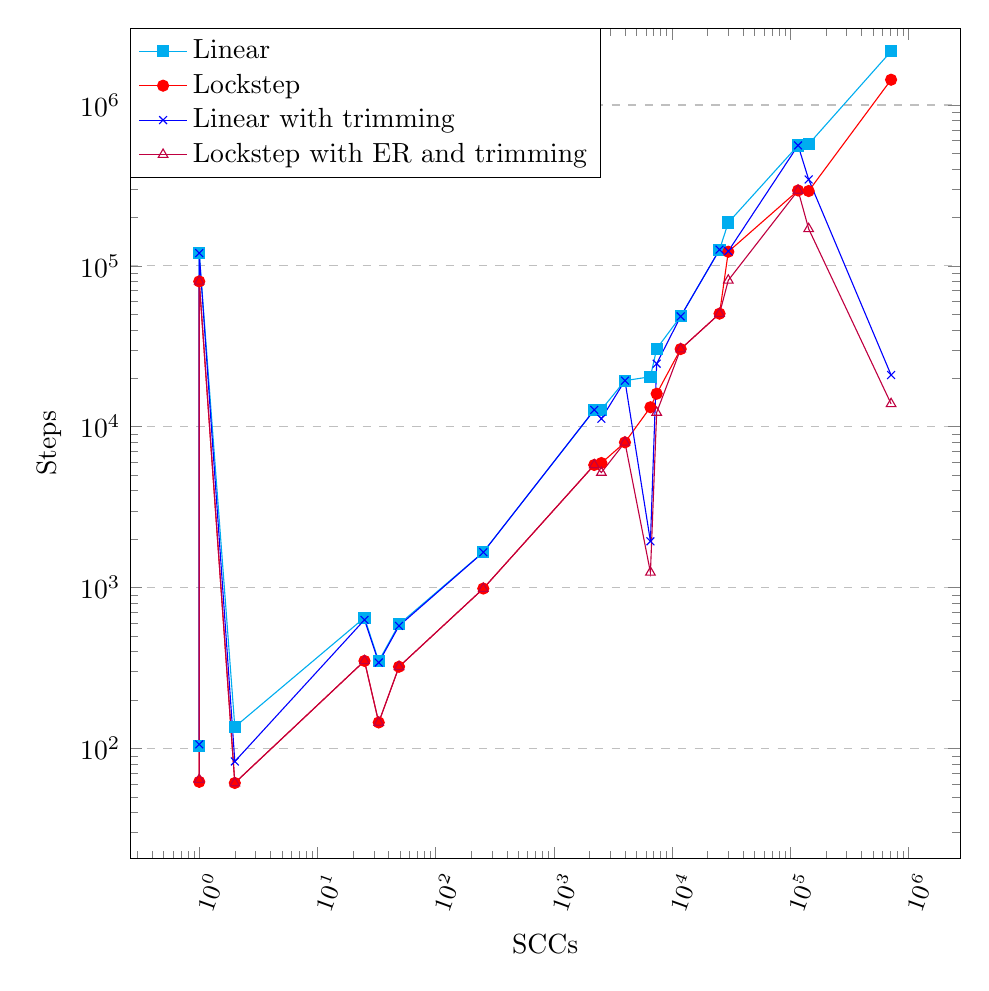
\begin{tikzpicture}
\begin{axis}[
height = \textwidth,
width=\textwidth,
x tick label style = {font = \small, align = center, rotate = 70, anchor = north east},
xlabel={SCCs},
ylabel={Steps},
ymin=0, ymax=3000000,
legend style={at={(0,1)},anchor=north west,legend cell align=left},
ymajorgrids=true,
grid style=dashed,
ymode=log,
log basis y={10},
xmode=log,
log basis x={10},
%xtick ={1, 1, 2, 25, 33, 49, 253, 2197, 2525, 3996, 6563, 7412, 11828, 25217, 29914, 116456, 143111, 713126}
]
\addplot[color=cyan,mark=square*,]coordinates {(1, 104)(1, 120017)(2, 136)(25, 650)(33, 349)(49, 591)(253, 1661)(2197, 12664)(2525, 12773)(3996, 19344)(6563, 20434)(7412, 30529)(11828, 48495)(25217, 126083)(29914, 185712)(116456, 560414)(143111, 570525)(713126, 2156545)};

\addplot[color=red,mark=*,]coordinates {(1, 62)(1, 80011)(2, 61)(25, 350)(33, 145)(49, 322)(253, 986)(2197, 5783)(2525, 5945)(3996, 7992)(6563, 13209)(7412, 16032)(11828, 30384)(25217, 50434)(29914, 122371)(116456, 294114)(143111, 291672)(713126, 1435356)};

\addplot[color=blue,mark=x,]coordinates {(1, 106)(1, 120019)(2, 83)(25, 630)(33, 342)(49, 578)(253, 1658)(2197, 12716)(2525, 11211)(3996, 19332)(6563, 1938)(7412, 24640)(11828, 48497)(25217, 126075)(29914, 123330)(116456, 560411)(143111, 344348)(713126, 20945)};
%\addplot[color=orange,mark=+,]coordinates {(1, 62)(1, 80011)(2, 61)(25, 350)(33, 145)(49, 322)(253, 986)(2197, 5783)(2525, 5945)(3996, 7992)(6563, 13209)(7412, 16032)(11828, 30384)(25217, 50434)(29914, 122371)(116456, 294114)(143111, 291672)(713126, 1435356)};
\addplot[color=purple,mark=triangle,]coordinates {(1, 64)(1, 80013)(2, 61)(25, 350)(33, 145)(49, 322)(253, 986)(2197, 5783)(2525, 5191)(3996, 7990)(6563, 1243)(7412, 12264)(11828, 30386)(25217, 50432)(29914, 81275)(116456, 294114)(143111, 169828)(713126, 13872)};
\legend{Linear, Lockstep, Linear with trimming, Lockstep with ER and trimming}
\end{axis}
\end{tikzpicture}
\caption{Steps performed compared to number of SCCs in graphs}\label{stepscc}
\end{figure}

\subsection{Diameter and SCCs vs. Steps}
Earlier on, we compared steps to nodes, but as the strengthened bound of $O(dN)$ on the number of symbolic steps is described in terms of diameter $d$ and number of SCCs $N$, we also decided to compare this with the number of steps. This can be seen in Figure \ref{dn}. We hoped that this would explain the outliers from Figure \ref{steps}.
\begin{figure}[h!]
  \centering
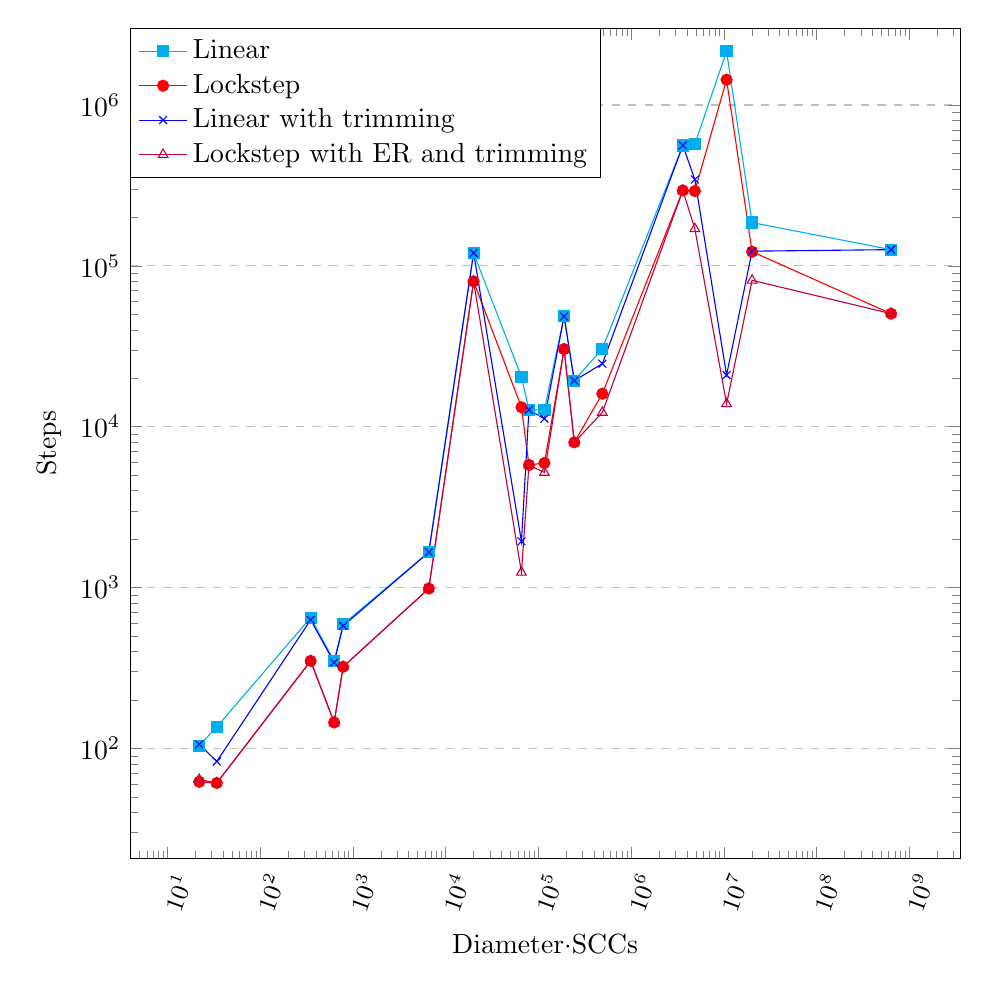
\begin{tikzpicture}
\begin{axis}[
height = \textwidth,
width=\textwidth,
x tick label style = {font = \small, align = center, rotate = 70, anchor = north east},
xlabel={Diameter$\cdot$SCCs},
ylabel={Steps},
ymin=0, ymax=3000000,
legend style={at={(0, 1)},anchor=north west,legend cell align=left},
ymajorgrids=true,
grid style=dashed,
ymode=log,
log basis y={10},
xmode=log,
log basis x={10}]
\addplot[color=cyan,mark=square*,]coordinates {(22, 104)(34, 136)(350, 650)(627, 349)(784, 591)(6578, 1661)(20003, 120017)(65630, 20434)(79092, 12664)(116150, 12773)(189248, 48495)(243756, 19344)(489192, 30529)(3610136, 560414)(4865774, 570525)(10696890, 2156545)(20162036, 185712)(635871872, 126083)};

\addplot[color=red,mark=*,]coordinates {(22, 62)(34, 61)(350, 350)(627, 145)(784, 322)(6578, 986)(20003, 80011)(65630, 13209)(79092, 5783)(116150, 5945)(189248, 30384)(243756, 7992)(489192, 16032)(3610136, 294114)(4865774, 291672)(10696890, 1435356)(20162036, 122371)(635871872, 50434)};

\addplot[color=blue,mark=x,]coordinates {(22, 106)(34, 83)(350, 630)(627, 342)(784, 578)(6578, 1658)(20003, 120019)(65630, 1938)(79092, 12716)(116150, 11211)(189248, 48497)(243756, 19332)(489192, 24640)(3610136, 560411)(4865774, 344348)(10696890, 20945)(20162036, 123330)(635871872, 126075)};
%\addplot[color=orange,mark=+,]coordinates {(22, 62)(34, 61)(350, 350)(627, 145)(784, 322)(6578, 986)(20003, 80011)(65630, 13209)(79092, 5783)(116150, 5945)(189248, 30384)(243756, 7992)(489192, 16032)(3610136, 294114)(4865774, 291672)(10696890, 1435356)(20162036, 122371)(635871872, 50434)};
\addplot[color=purple,mark=triangle,]coordinates {(22, 64)(34, 61)(350, 350)(627, 145)(784, 322)(6578, 986)(20003, 80013)(65630, 1243)(79092, 5783)(116150, 5191)(189248, 30386)(243756, 7990)(489192, 12264)(3610136, 294114)(4865774, 169828)(10696890, 13872)(20162036, 81275)(635871872, 50432)};
\legend{Linear, Lockstep, Linear with trimming, Lockstep with ER  and trimming}
\end{axis}
\end{tikzpicture}
\caption{Steps compared to the strengthened bound}\label{dn}
\end{figure}

\subsection{something something worst-case performance}

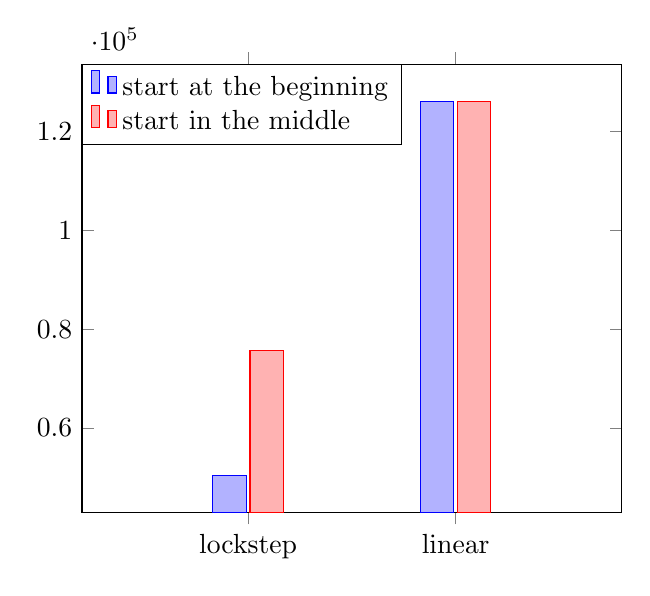
\begin{tikzpicture}
 
\begin{axis} [ybar = .05cm,
    bar width = 12pt,
    enlarge x limits = {abs = .8},
    xtick={1,2},
    xticklabels={lockstep, linear},
    legend style={at={(0, 1)},anchor=north west,legend cell align=left},
]

\addplot coordinates {(1, 50434) (2, 126083)};
\addplot coordinates {(1, 75652) (2, 126079)};
 
\legend {start at the beginning, start in the middle};
 
\end{axis}
 
\end{tikzpicture}

\end{document}
%%% Local Variables:
%%% mode: latex
%%% TeX-master: "../master/master"
%%% End:
